\documentclass[tikz, convert]{standalone}
\usepackage{amsmath} % for aligned

\usetikzlibrary{positioning, calc, decorations.pathreplacing}

\begin{document}
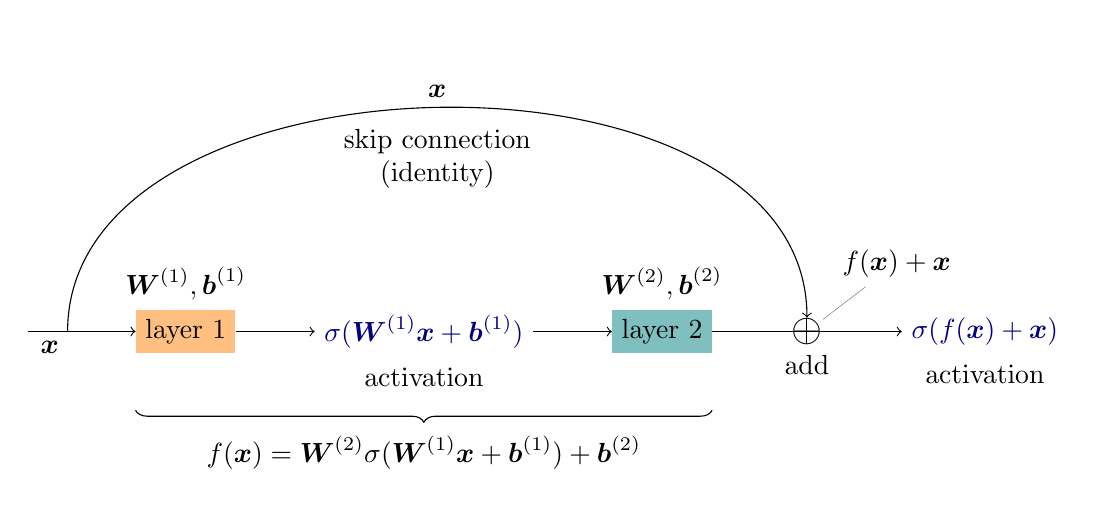
\begin{tikzpicture}

  \node[fill=orange!50, label={above:$\boldsymbol{W}^{(1)}, \boldsymbol{b}^{(1)}$}] (l1) {layer 1};
  \node[blue!50!black, right=of l1, label={below:activation}] (act1) {$\sigma(\boldsymbol{W}^{(1)}\boldsymbol{x} + \boldsymbol{b}^{(1)})$};
  \node[fill=teal!50, right=of act1, , label={above:$\boldsymbol{W}^{(2)}, \boldsymbol{b}^{(2)}$}] (l2) {layer 2};
  \node[right=of l2, font=\Large, label={below:add}, inner sep=0, pin={60:$f(\boldsymbol{x}) + \boldsymbol{x}$}] (add) {$\oplus$};
  \node[blue!50!black, right=of add, label={below:activation}] (act2) {$\sigma(f(\boldsymbol{x}) + \boldsymbol{x})$};

  \draw[->] (l1) -- (act1);
  \draw[->] (act1) -- (l2);
  \draw[<-] (l1) -- ++(-2,0) node[below, pos=0.8] {$\boldsymbol{x}$};
  \draw[->] (l2) -- (act2) node[above, pos=0.8] {};
  \draw[->] ($(l1)-(1.5,0)$) to[out=90, in=90] node[below=1ex, midway, align=center] {skip connection\\(identity)} node[above, midway] {$\boldsymbol{x}$} (add);
  \draw[decorate, decoration={brace, amplitude=1ex, raise=1cm}] (l2.east) -- node[midway, below=1.2cm] {$f(\boldsymbol{x}) = \boldsymbol{W}^{(2)}\sigma(\boldsymbol{W}^{(1)}\boldsymbol{x} + \boldsymbol{b}^{(1)}) + \boldsymbol{b}^{(2)}$} (l1.west);

\end{tikzpicture}
\end{document}